%version of 02-28-20

\chapter{The hidden ordering of numbers}
\label{Appendix:Tetra}

Our objective here is to develop the reasoning which leads to a proof...

\section{Revisiting tirangular numbers}

\begin{figure}[h]
\begin{center}
        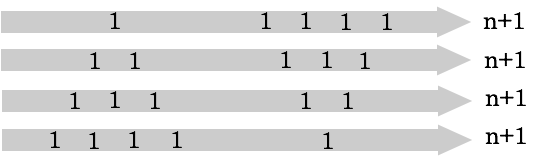
\includegraphics[scale=0.4]{FiguresArithmetic/appTetrahedral2}
        \caption{Computing $\Theta_n$: basic triangle pattern.}
        \label{fig:Tetrahedral2}
\end{center}
\end{figure}

\section{Tetrahedral numbers}
\label{sec:tetraedralNumbers}

Prove the following expression

$\Theta_n =  \sum_{k=1}^{n} \Delta_k = \frac{n.(n+1).(n+2)}{6}$
\medskip


This result can easily been proved by recurrence, we let the reader develop it. 
We suggest to use the double counting Fubini's principle.

Following this way, you should write the previous expression of the tetrahedral number in a developed form 
using a triangle shape as shown in Fig.~\ref{fig:Tetrahedral2}.

and draw two copies by rotating the dimensions.

Fubini's principle is used by summing up the successive rows.

Prove as an intermediate result that the sum of the elements over the rows of the three triangles is proportional to $n+2$.
\medskip

\noindent \textit{The detailed solution.}
We proved the expression of $\Delta_n$ by mirroring the developed expression and adding term by term.
Similarly, a way to prove the expression of $\Theta_n$ is to consider three copies and organize them 
in order to obtain the expected result.
A tetrahedral number can be arranged as a triangle (see Fig.~\ref{fig:TetrahedralBasic}).
%\begin{figure}[h]
%\begin{center}
%        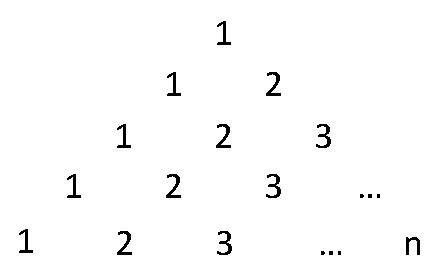
\includegraphics[scale=0.5]{FiguresArithmetic/TetrahedralBasic}
%        \caption{Computing $\Theta_n$: basic triangle pattern.}
%        \label{fig:TetrahedralBasic}
%\end{center}
%\end{figure}

The proof is obtained by the double counting principle by rotating the three faces of triangles as shown in Fig.~\ref{fig:Tetrahedral}.
\begin{figure}[h]
\begin{center}
        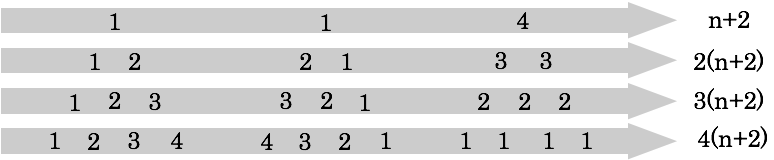
\includegraphics[scale=0.3]{FiguresArithmetic/appTetrahedral3}
        \caption{Computing $\Theta_n$: basic triangle pattern.}
        \label{fig:Tetrahedral3}
\end{center}
\end{figure}

\begin{figure}[h]
\begin{center}
        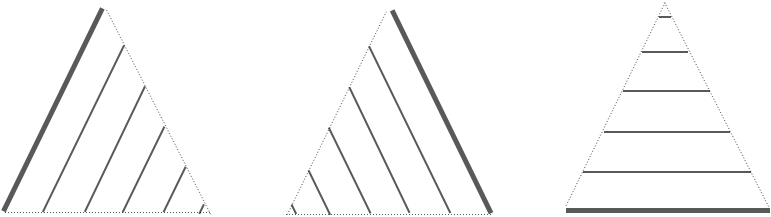
\includegraphics[scale=0.3]{FiguresArithmetic/appTetrahedral1}
        \caption{Computing $\Delta_n$: basic triangle pattern.}
        \label{fig:Tetrahedral1}
\end{center}
\end{figure}


Sum up all the numbers in each row.

\begin{itemize}
\item 
The first row is equal to $1+1+n = n+2$.
\item
The second one is equal to $3 + 3 + 2(n-1) = 2(n+2)$. 
\item
Let us sum up the elements in row $k$: 

$\Delta_k + \Delta_k + k(n-k+1)  = k(k+1) + kn-k^2+k = k(n+2)$.
\end{itemize}

Conclusion:
the global sum is equal to $n+2$ times $(1+2+...+n)$.

Finally, $3 \Theta_n = (n+2) \Delta_n$.
\medskip

\noindent \textit{Going further.}

Summary: we proved the following results:
\begin{itemize}
\item $Id_n = 1+1+ ... +1 = n$
\item $\Delta_n = 1+2+3+ ... +n = \frac{1}{2}.Id_n.(n+1)$
\item $\Theta_n = \Delta_1 + \Delta_2 + ... + \Delta_n = \frac{1}{3} .\Delta_n.(n+2)$
\end{itemize}


\section{Pentahedral numbers}

A natural question is if we can go further following the same pattern for computing 
$ \sum_{k=1}^{n} \Theta_k$, and so on.

\begin{figure}[h]
\begin{center}
        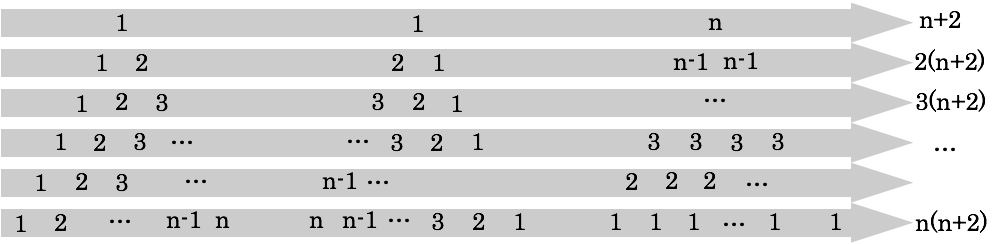
\includegraphics[scale=0.3]{FiguresArithmetic/appTetrahedral4}
        \caption{Computing $\Theta_n$: basic triangle pattern.}
        \label{fig:Tetrahedral4}
\end{center}
\end{figure}

\begin{figure}[h]
\begin{center}
        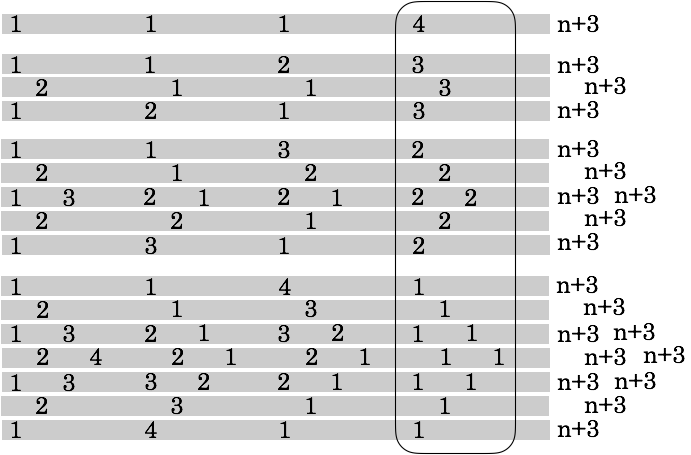
\includegraphics[scale=0.4]{FiguresArithmetic/appTetrahedral5}
        \caption{Computing $\Theta_n$: basic triangle pattern.}
        \label{fig:Tetrahedral5}
\end{center}
\end{figure}

\begin{figure}[h]
\begin{center}
        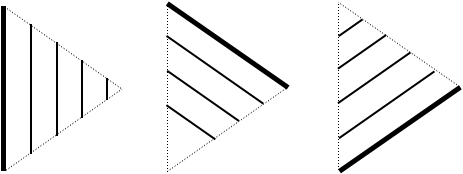
\includegraphics[scale=0.35]{FiguresArithmetic/appTetrahedral6}
        \caption{Computing $\Theta_n$: basic triangle pattern.}
        \label{fig:Tetrahedral6}
\end{center}
\end{figure}

Are you able to consider the challenge?



